\documentclass[tikz,border=5pt]{standalone}
\usetikzlibrary{shapes.geometric}
\begin{document}
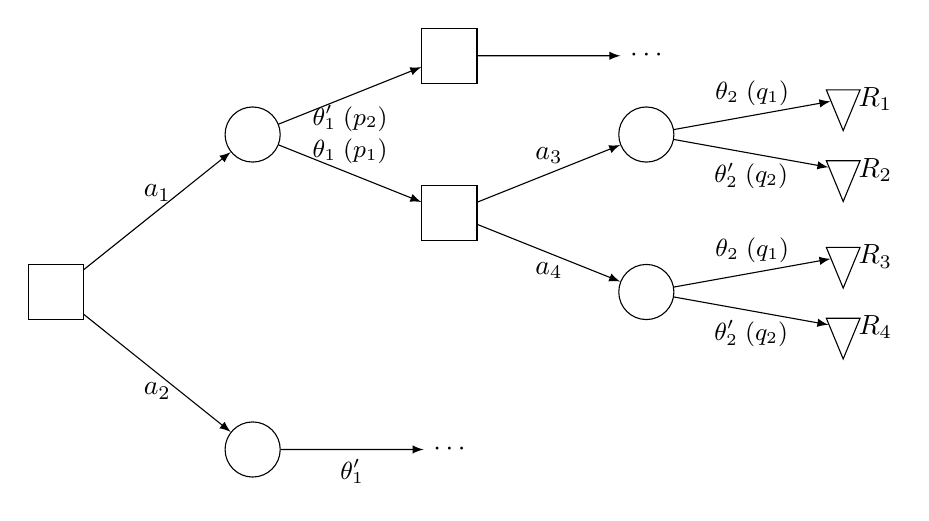
\begin{tikzpicture}[
  grow=right, level distance=2.5cm, sibling distance=1cm,
  decision/.style={rectangle, draw, minimum size=7mm},
  chance/.style={circle, draw, minimum size=7mm},
  terminal/.style={isosceles triangle, draw, shape border rotate=-90, minimum height=5mm, minimum width=3mm},
  edge from parent/.style={draw, -latex},
  level 1/.style={sibling distance=4cm},
  level 2/.style={sibling distance=2cm},
  level 3/.style={sibling distance=2cm},
  level 4/.style={sibling distance=0.9cm}
]
\node [decision] {}
  child {node [chance] {}
    child {node {$\cdots$} edge from parent node[below] {\small $\theta_1'$}}
    edge from parent node[below] {$a_2$}
  }
  child {node [chance] {}
    child {node [decision] {}
      child {node [chance] {}
        child {node [terminal] {} node[right=2pt] {$R_4$}
          edge from parent node[below] {\small $\theta_2'\;(q_2)$}}
        child {node [terminal] {} node[right=2pt] {$R_3$}
          edge from parent node[above] {\small $\theta_2\;(q_1)$}}
        edge from parent node[below] {$a_4$}
      }
      child {node [chance] {}
        child {node [terminal] {} node[right=2pt] {$R_2$}
          edge from parent node[below] {\small $\theta_2'\;(q_2)$}}
        child {node [terminal] {} node[right=2pt] {$R_1$}
          edge from parent node[above] {\small $\theta_2\;(q_1)$}}
        edge from parent node[above] {$a_3$}
      }
      edge from parent node[above] {\small $\theta_1\;(p_1)$}
    }
    child {node [decision] {}
      child {node {$\cdots$} edge from parent}
      edge from parent node[below] {\small $\theta_1'\;(p_2)$}
    }
    edge from parent node[above] {$a_1$}
  };
\end{tikzpicture}
\end{document}
